\chapter{Элементы нотной грамоты}
\label{ch:note}

Нотную запись нельзя назвать эталоном простоты. Она, несомненно, сложнее, чем могла бы быть. Так уж сложилось, и, уважая гениальность предков, мы изучим её такой, какая она есть.


\section{Немного теории}

\emph{Нота} --- это \emph{обозначение} (способ записи, если хотите) колебаний воздуха с некоторой постоянной частотой. Такие колебания некоторое время производит гитарная струна после щипка --- особого удара пальцем по ней. Нота звучит \emph{выше}, если частота колебаний струны \emph{больше}. Ну а низкая нота --- это колебания с малой частотой. Например, в соответствии с международным стандартом, струна, звучащая на ноте Ля первой октавы (о октавах позже) колеблется с частотой 440 герц, то есть совершает 440 полных колебаний в секунду\footnote{Допускается вольность принять за Ля первой октавы любую частоту из интервала от 430 до 450 герц. Многие фанатики утверждают, что Ля в 432 Гц от Бога (и оздоравливающе действует на организм), а стандартизованная 440 Гц --- от Сатаны, соответственно (и разрушает психику).}.

Человеческое ухо способно различать такие характеристики звуковой волны, как её частота и амплитуда. Незатухающие колебания одной неизменной частоты, человек услышит как тон\footnote{Например, заходящий на посадку на ваше ухо комар, машет крыльями примерно 659.26 раз в секунду и вы слышите незабываемое Ми второй октавы!}. А амплитуду волны (размах колебаний) --- как громкость. Человеческий слуховой аппарат воспринимает ограниченный диапазон частот (примерно от 16 до 20000 Гц), а восприятие громкости звука, если честно, зависит не только от амплитуды звуковых колебаний, но и от частоты.

В Русской традиции принято использовать \emph{семь} обозначений для кодирования нот (которые приведены ниже в порядке возрастания частоты колебаний (высоты звука)): 
\begin{center}
    До, Ре, Ми, Фа, Соль, Ля, Си. 
\end{center}

Так что получается, мы имеем дело всего с семью звуками? Конечно нет!

Пусть мы дошли до последней ноты Си и... И текущая \emph{октава} кончилась. Но началась следующая! В следующей октаве все повторится: До, Ре, Ми, Фа, Соль, Ля, Си. Только вот частота соотвествующей ноты будет в \emph{два} раза больше! То есть, например, ноте Ля второй октавы соответствует вдвое большая частота (880 Гц), чем ноте Ля первой октавы (стандартные 440 Гц).

Октавы, использующиеся в музыке, имеют следующие названия.
\begin{center}
    \begin{tabular}{ll}
        \hline\hline
        Название октавы         & Частота ноты Ля, Гц \\
        \hline\hline
        
        Субконтроктава          & 27.5 \\
        Контроктава             & 55   \\
        \emph{Большая октава}   & 110  \\
        \emph{Малая октава}     & 220  \\
        \emph{Первая октава}    & \fbox{440}  \\
        \emph{Вторая октава}    & 880  \\
        Третья октава           & 1760 \\
        Четвертая октава        & 3520 \\
        Пятая октава            & 7040 \\
        \hline
    \end{tabular}
\end{center}

В таблице \emph{выделены} те октавы, которые входят в диапазон шестиструнной гитары. Справедливости ради следует сказать, диапазон звучания гитары полностью включает лишь малую и первую октавы.

А вот теперь пришло время для секретов: традиционно в октаве принято выделять \emph{двенадцать} нот! 

Погодите, погодите, скажете вы: <<До, Ре, Ми, Фа, Соль, Ля, Си>> --- семь нот! И октава названа, вероятно, не просто так: <<octo>> --- это восемь, восьмая нота! Все логично!

Сам в шоке! Но увы, <<До, Ре, Ми,\ldots>> --- это названия лишь семи нот из 12. А вот (12-7)=5 нот не удостоились отдельных имен. Итак, оставшиеся 5 нот находятся между упорядоченными по частоте нотами:
\begin{enumerate}
    \item До и Ре (эта нота может быть названа либо До-диез, либо Ре-бемоль)
    \item Ре и Ми (Ре-диез или Ми-бемоль)
    \item Фа и Соль (Фа-диез или Соль-бемоль)
    \item Соль и Ля (Соль-диез или Ля-бемоль)
    \item Ля и Си (Ля-диез или Си-бемоль)
\end{enumerate}    

Эти <<промежуточные>> ноты имеют сразу два названия. Все 12 нот октавы в порядке увеличения высоты:
\begin{center}
    До, \emph{До-диез}, Ре, \emph{Ре-диез}, Ми, Фа, \emph{Фа-диез}, Соль, \emph{Соль-диез}, Ля, \emph{Ля-диез}, Си
\end{center}

Частота от ноты к ноте повышается равномерно, в \emph{геометрической} прогрессии. Частота каждой следующей ноты в \[\sqrt[12]{2}\approx 1,059463\] больше частоты предыдущей. 

Так, следующая за нотой Ля первой октавы, нота Ля-диез, имеет частоту $440\cdot\sqrt[12]{2}\approx 466,16$ герц. Нота Си имеет частоту $440\cdot(\sqrt[12]{2})^2\approx 493,88$. И так далее, например, Ля второй октавы имеет в два раза большую частоту, чем Ля первой октавы: $440\cdot(\sqrt[12]{2})^{12}=440\cdot 2=880$ Гц.

Задав эталонную частоту любой ноты, частоты для всех остальных нот можно вычислить.

В учебниках говорится, что добавление суффикса <<диез>> означает повышение частоты исходной ноты на <<полутон>>, что математически соответствует увеличению частоты в $\sqrt[12]{2}$ раз. И это в целом правильно, только обычно ученики начинают думать, что между соседними нотами из списка До, Ре, Ми, Фа, Соль, Ля, Си --- расстояние в два <<полутона>> (то есть в <<тон>>)! Не забыайте, что между нотами Ми и Фа, а также между Си и До <<промежуточных>> нот нет и расстояние между ними --- один <<полутон>>. 

Как видно из реальной последовательности, следуя такой логике, например, Ми-диез --- это Фа, или Си-диез --- это До следующей октавы. Обычно ноту Фа, конечно никто не называет Ми-диез --- это оскорбительно, но никто и не запрещает так делать. 

То же самое можно сказать и о суффиксе <<бемоль>>, он понижает ноту на полтона. И, например, До-диез, это та же нота, что и Ре-бемоль. А если вы хотите оскорбить ноту Ми, то назовите её Фа-бемоль. Если вы хотите прочитать все 12 нот в обратном порядке, то грамотно будет использовать суффикс <<бемоль>>, а не <<диез>>:

\begin{center}
Си, Си-бемоль, Ля, Ля-бемоль, Соль, Соль-бемоль, Фа, Ми, Ми-бемоль, Ре, Ре-бемоль, До.
\end{center}


\section{Устройство гитары}

Мы разобрались с теорией нот в предыдушем разделе, теперь коснемся особенностей устройства гитары, которые позволяют извлекать ноты именно такими, какими они и должны быть. 

Для начала стоит взглянуть на рисунок \ref{fig:guitarConstruction} и запомнить, что значат незнакомые вам обозначения.

\begin{figure}[!ht]
    \centering
    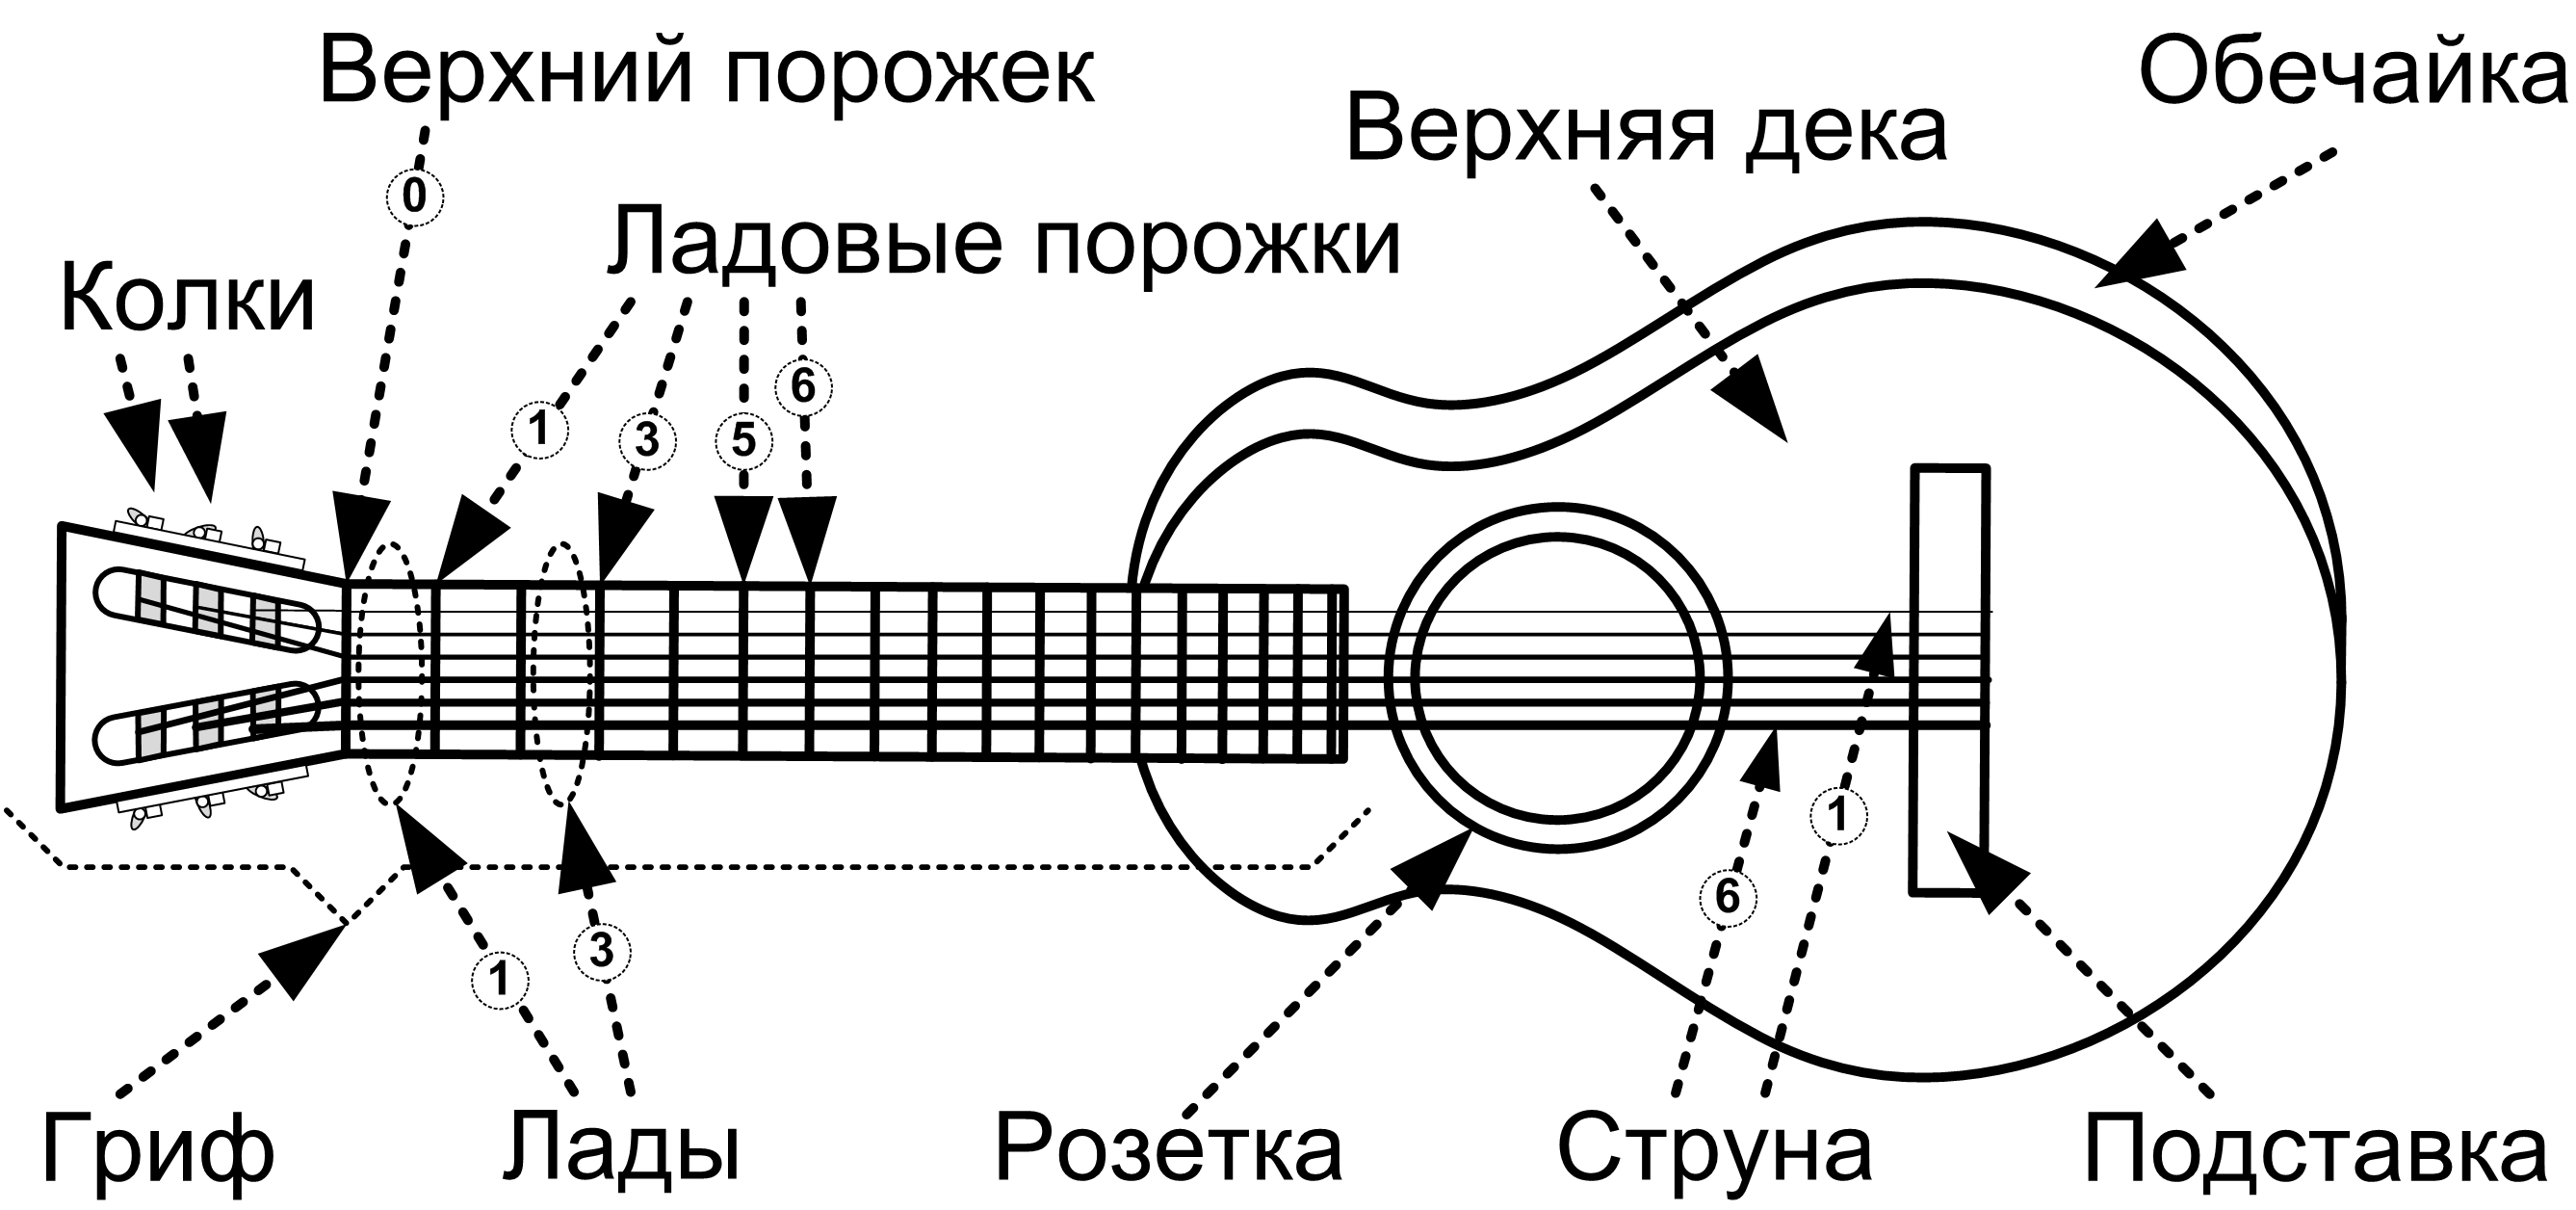
\includegraphics{fig/guitar-construction} 
    \caption{Устройство гитары}\label{fig:guitarConstruction}
\end{figure} 

Любая открытая\footnote{То есть не зажатая ни на каком ладу} струна гитары звучит строго определенной нотой (о настройке гитары поговорим позже). Лады на грифе (промежутки между порожками), равно как и \emph{ладовые порожки} считаются от \emph{верхнего} порожка: 1,2,3,\ldots и т.д. То есть <<зажать струну на первом ладу>> значит, что вы ставите палец на струну, на первый лад, то есть между верхним порожком и первым ладовым\footnote{Чем ближе к первому ладовому, тем лучше. Таким образом и звук будет чище, и рука уставать будет меньше. Ставить палец сверху на порожек не стоит --- звук будет <<глохнуть>>. Правда иногда именно это и требуется. Но в начале обучения стоит ставить палец на ладу ближе к тому порожку, от которого идет <<звучащая>> часть струны. Добивайтесь чистого звука.} и нажимаете до тех пор, пока струна не прижмётся к первому ладовому порожку. Но нам важно сейчас не то, как правильно зажимать струну. 

Важно понять, что каждый следующий лад понижает звук на струне на <<полтона>>. В октаве 12 нот и каждая звучит на струне на своём ладу. На дветадцатом ладу звучит нота открытой струны, но выше на октаву.

Из физики известно, что частота колебаний струны обратно пропорциональна её длине\footnote{Надо честно заметить, что частота колебаний струны зависит также и от силы её натяжения, которая меняется, когда струну <<зажимают>> на ладу. Но это влияние столь незначительно, что им можно пренебречь.}. Стало быть, чтобы частота издаваемого струной звука \emph{увеличилась} вдвое (а языком музыки --- чтобы нота зазвучала октавой выше), надо вдвое \emph{укоротить} струну. 

Зажимая струну на 12 ладу (языком музыки --- повышая ноту открытой струны на октаву), вы укарачиваете струну вдвое. Линейка в помощь, если не верите\footnote{Конечно нужно мерять только звучащую (колеблющуюся часть) струны от опоры на подставке до порожка.}.

Конечно, частота колебаний струны зависит также и от силы её натяжения. Сила натяжения струны регулируется колками на грифе, когда гитару настраивают. Играя, гитарист только меняет длину звучащего участка струны, зажимая струны на ладах. Редкие психи\footnote{Конечно, имелось в виду: \emph{мастера}! Прим. ред.} крутят колок во время исполнения, добиваясь сомнительных\footnote{Конечно, имелось в виду: \emph{удивительных}! Прим. ред.} эффектов.

Исходя из того, что частота каждой следующей ноты в $\sqrt[12]{2}$ больше предыдущей, запишем формулу длины струны ($L$) от места крепления струны к подставке до $n$-го ладового порожка:

\[L(n)=\frac{L}{(\sqrt[12]{2})^n},\]
где $n$ - номер лада ($0$-й лад соответствует открытой струне), а $L$ --- общая длина струны от подставки до верхнего порожка.


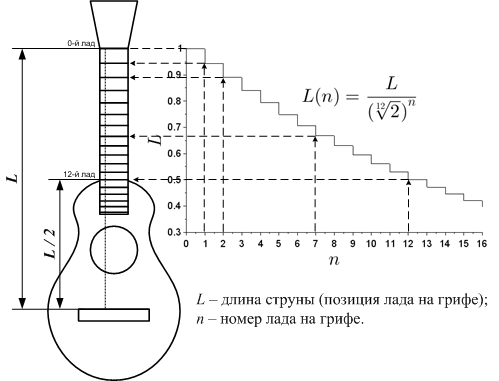
\includegraphics{fig/string-length.png}

Ушастые выпендрёжники говорят, что различают больше 12 нот в октаве! И им мало 12 ладов! На некоторых гитарах можно заметить дополнительные ладовые порожки между <<каноническими>>, которые позволяют <<всунуть>> дополнительную ноту.


\section{Запись гитарных нот на бумаге}

\section{Поиск нот на грифе}

\begin{figure}[!ht]
    \centering
    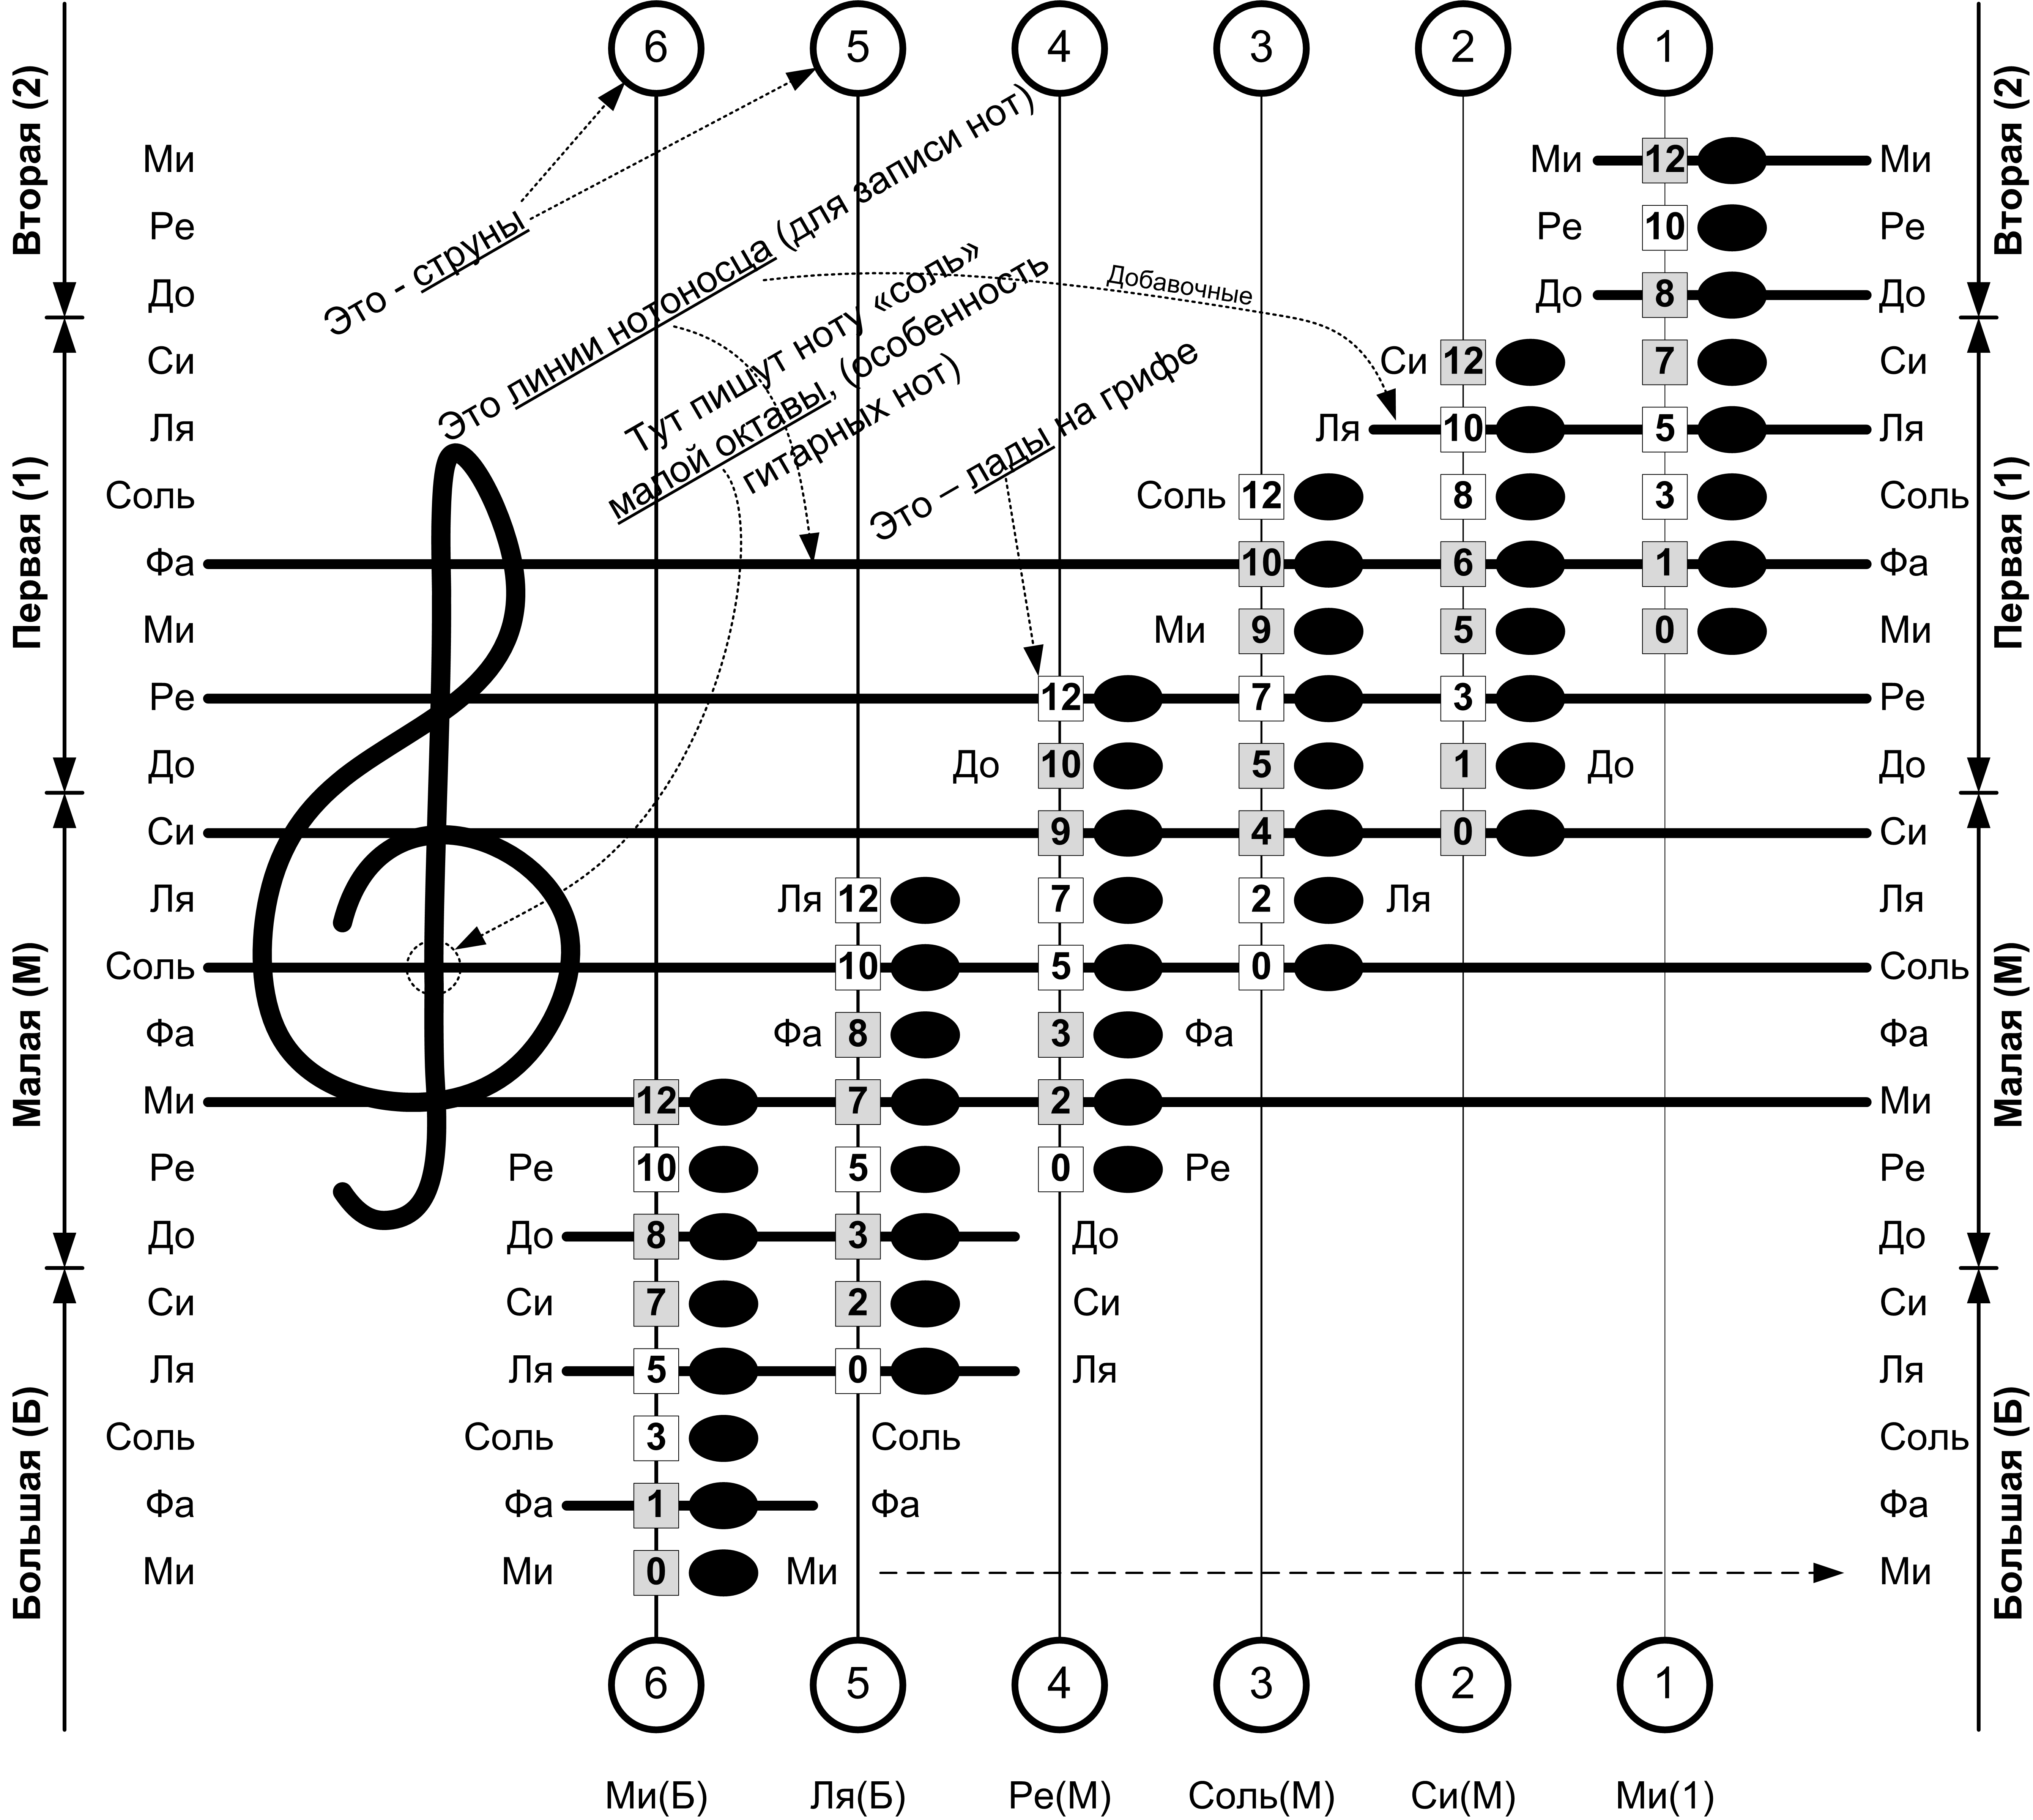
\includegraphics[width=\textwidth]{fig/lad-by-notes} 
    \caption{Ноты на грифе (гриф поперек нотоносца)}\label{fig:ladByNotes}
\end{figure} 

\begin{figure}[!ht]
    \centering
    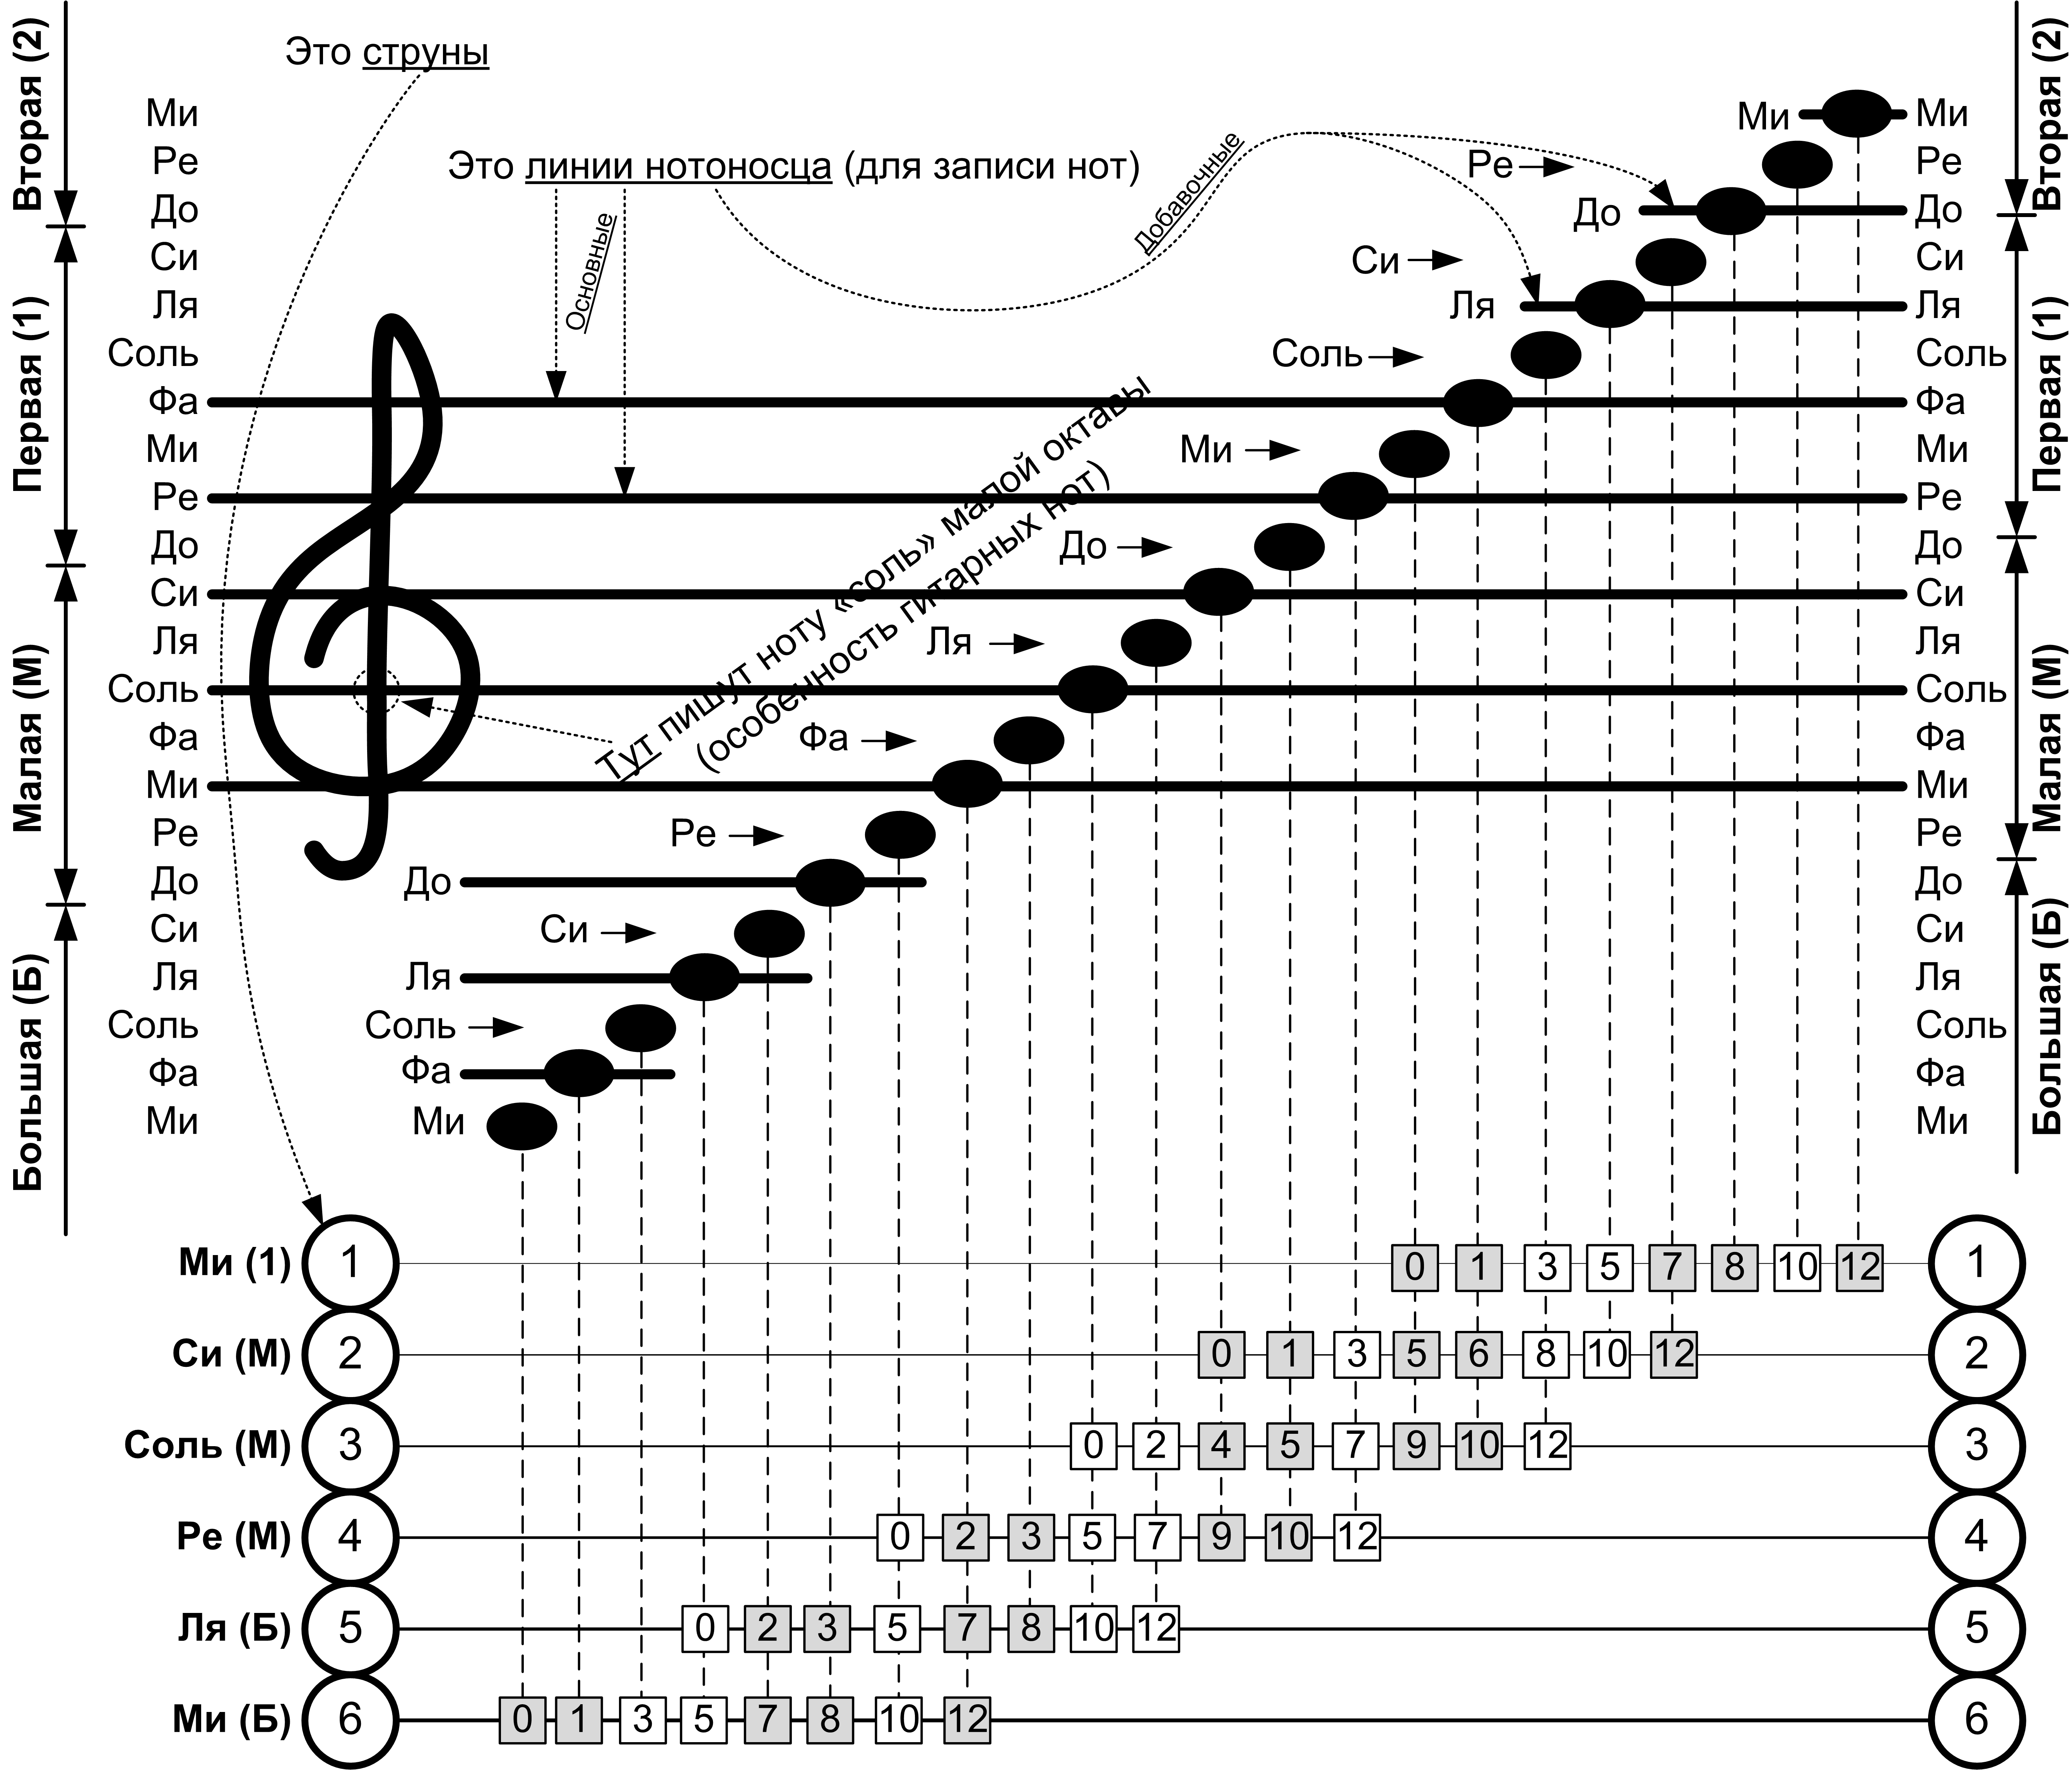
\includegraphics[width=\textwidth]{fig/lad-by-griph} 
    \caption{Ноты на грифе (гриф вдоль нотоносца)}\label{fig:ladByGriph}
\end{figure} 

\begin{figure}[!ht]
    \centering
    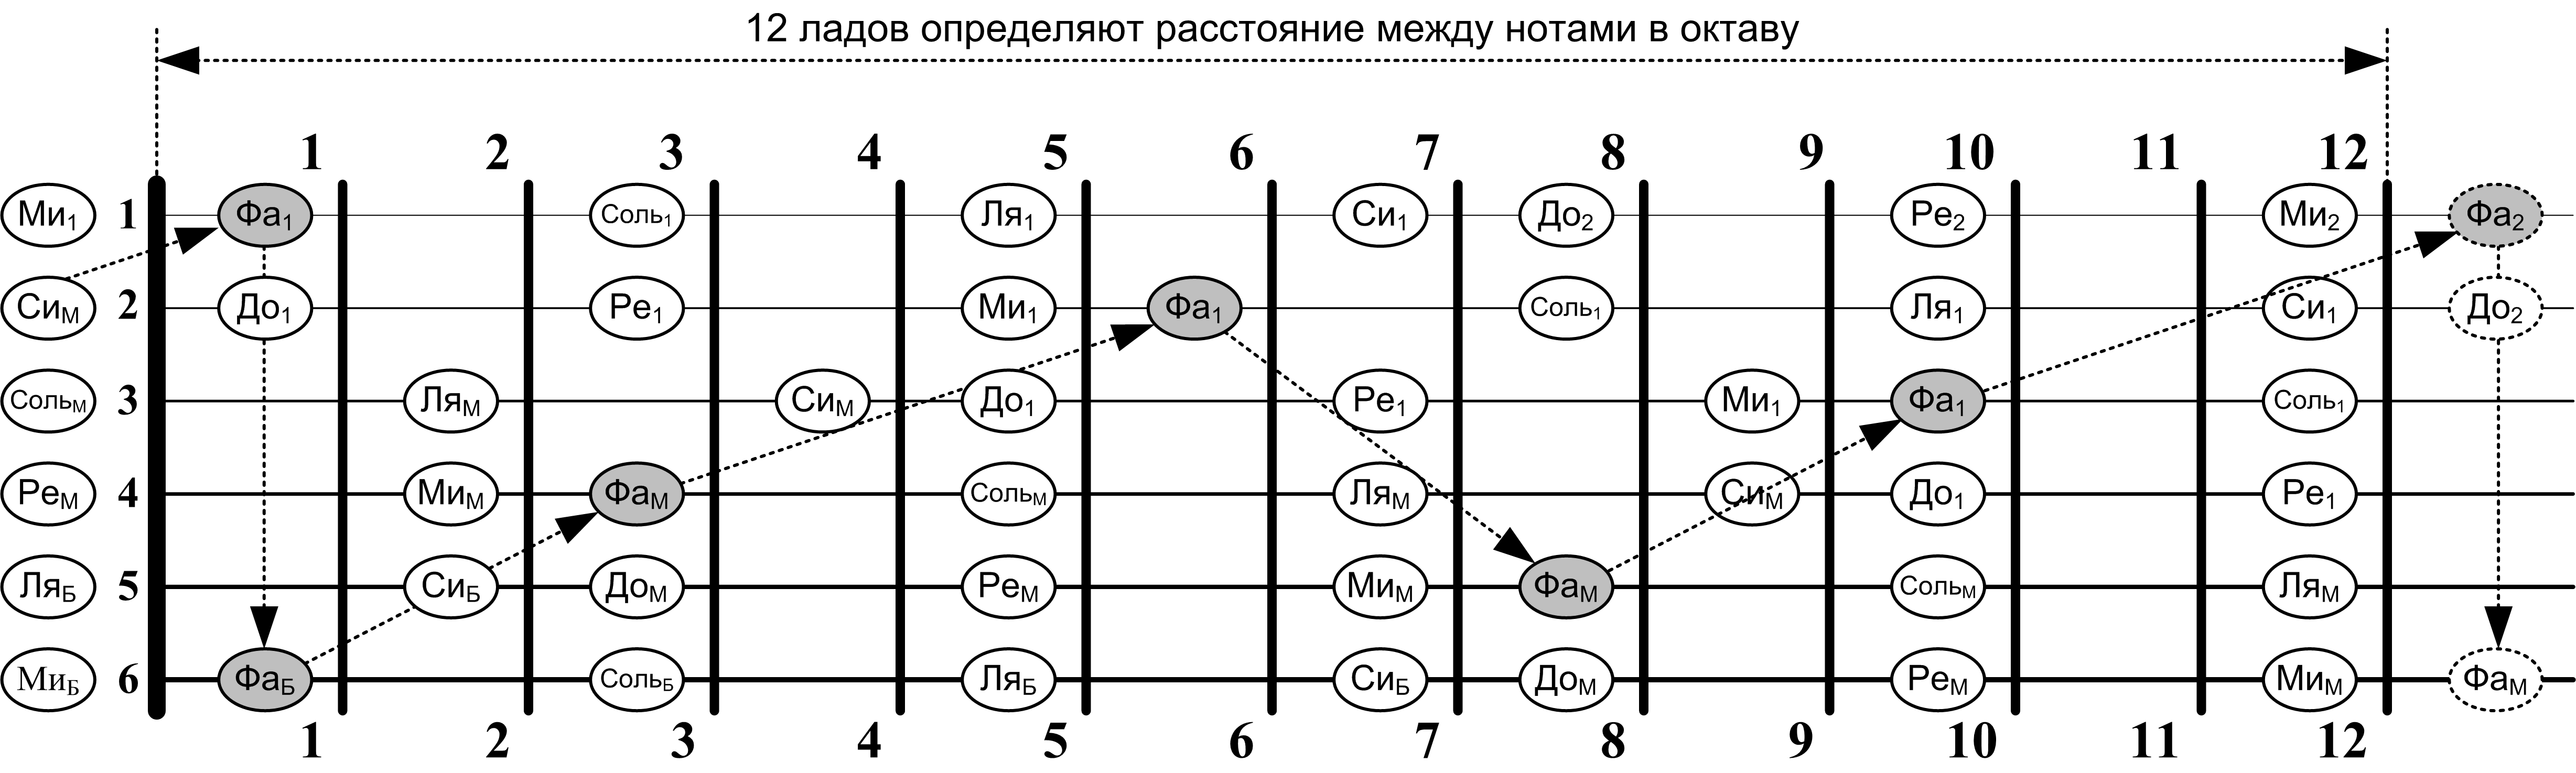
\includegraphics[width=\textwidth]{fig/notes-on-griph} 
    \caption{Ноты на грифе (относительное расположение)}\label{fig:notesOnGriph}
\end{figure} 


\section{Гитарная табулатура}

